%!TEX root = ../dokumentation.tex

\chapter{Stand der Technik}
\section{Mikrocontroller}
\label{sec:Mikrocontroller}
Unter einem Mikrocontroller versteht man einen kleinen, eigenständigen Computer. Sie bestehen aus einem Prozessor, Speicher und Ein-/Ausgabefunktionen und sind speziell für die Steuerung von elektronischen Geräten und Systemen entwickelt \protect\citeM{i}{Bernstein_Herbert.2020}{2}{2}.

\subsection{ESP8266}
\label{subsec:ESP8266}
Projektvorgabe war die Arbeit mit einem sogenannten ESP8266, oder einem vergleichbaren Mikrocontroller. Der ESP8266 ist ein spezieller Mikrocontroller, welcher sich besonders durch eine erhöhte Rechenleistung und einen integrierten \ac{WLAN}-Chip für einen vergleichsweise geringen Preis auszeichnet \protect\citeM{i}{Cameron_Neil.2021}{Preface}{Preface}.

\section{Abstandssensoren}
Abstandssensoren sind Sensoren, welche zur Ermittlung der Distanz zwischen zwei Punkten verwendet werden. Im Laufe der Zeit wurden verschiedenste Sensoren entwickelt, um das zu ermöglichen. Zu den bekanntesten Abstandssensoren gehören beispielsweise der Ultraschallsensor, sowie auch der Infratotsensor.
Der Grundgedanke hinter der Abstandsermittlung mit einem dieser beiden Sensoren wurde von der Fledermaus adaptiert. Diese sendet Schallwellen im für Menschen nicht hörbaren Bereich aus. Wenn ein Gegenstand die Schallwellen reflektiert, so kommen diese wieder bei der Fledermaus an und diese kennt die Richtung und den ungefähren Abstand zum Objekt. So kann sie ihre Beute und potentielle Hindernisse in der Flugbahn selbst bei absoluter Dunkelheit ausfindig machen.

\begin{figure}[H]
	\centering
	\resizebox{.9\textwidth}{!}{%
		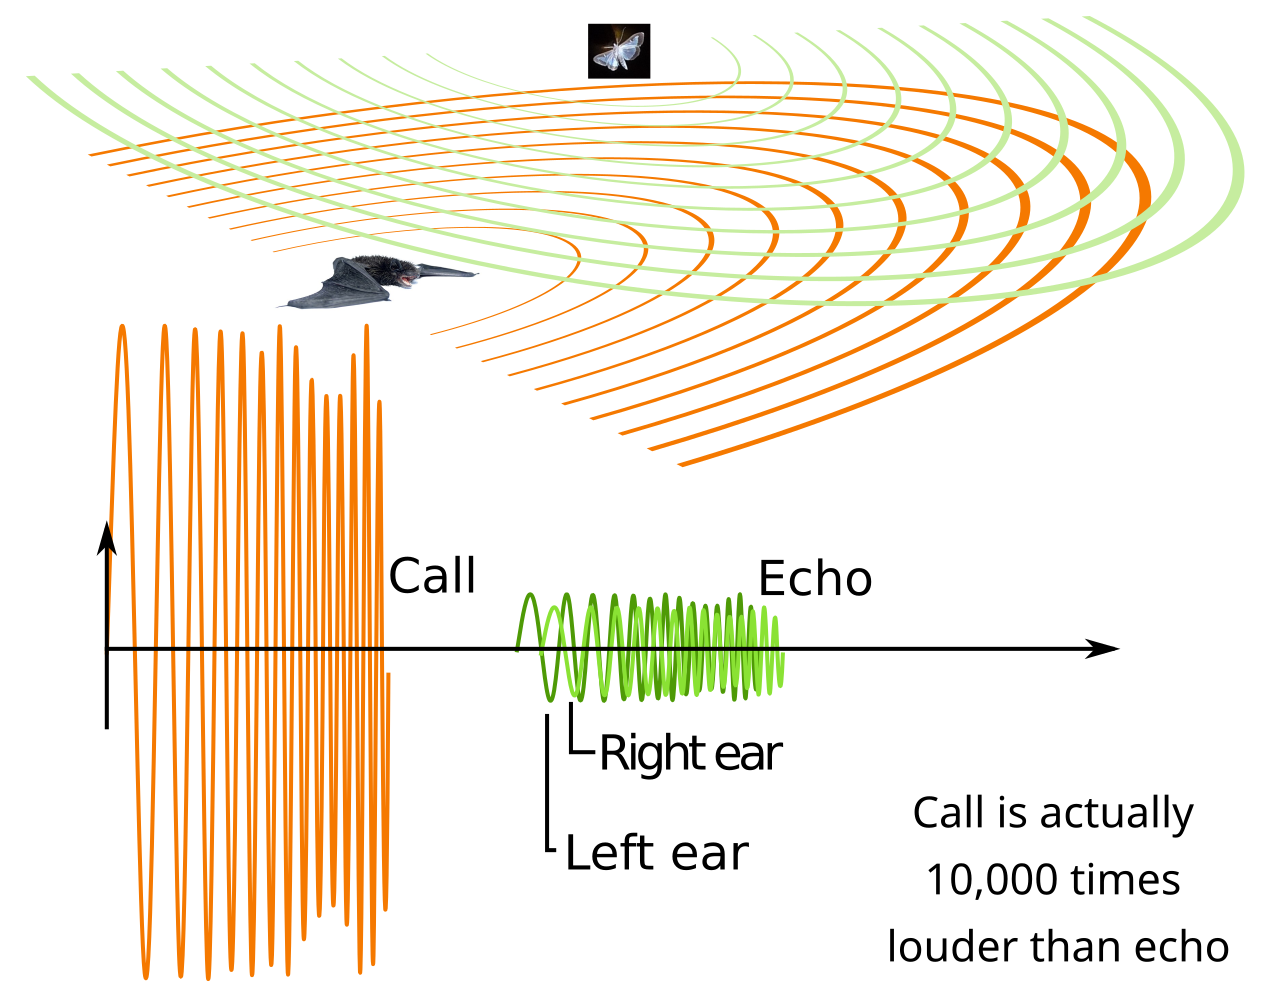
\includegraphics{images/Bat_Echo.png}
	}
	\caption[Ultraschallwellen einer Fledermaus]{Animal Echolocation, \protect\citeM{i}{Aimonen_Petteri.2009}{}{}} \label{fig:withSource} % Wie gebe ich hier die Quelle an?
\end{figure}

Wie auch bei der Fledermaus senden die beiden Sensortypen ein Signal aus und messen dessen Rückkehr nach der Kollision mit einem Gegenstand. Wenn die Ausbreitungsgeschwindigkeit des entsprechenden Signals bekannt ist, so kann die zurückgelegte Distanz und somit auch die Entfernung zum Gegenstand ermittelt werden. Unterscheiden tun sich die Sensortypen lediglich in der Art des ausgesendeten Signals. Der Ultraschallsensor sendet, wie der Name schon sagt, Ultraschallwellen aus \protect\citeM{i}{Thomas_Christian.1965}{126}{126}, \protect\citeM{i}{Tille_Thomas.2016}{499}{500}. Der Infrarotsensor entsprechend Infrarotwellen \protect\citeM{i}{Thomas_Christian.1965}{127}{127}.


\subsection{Der HC-SR04 Ultraschallsensor}
Im Rahmen dieses Projektes wurde für die Abstandsmessung ein vergleichsweise günstiger Entfernungssensor verwendet. Dieser hat eine Breite von 4,5 cm und ohne einberechnung der Pins eine Höhe von 2 cm.

\begin{figure}[h!]
	\centering
	\resizebox{.9\textwidth}{!}{%
		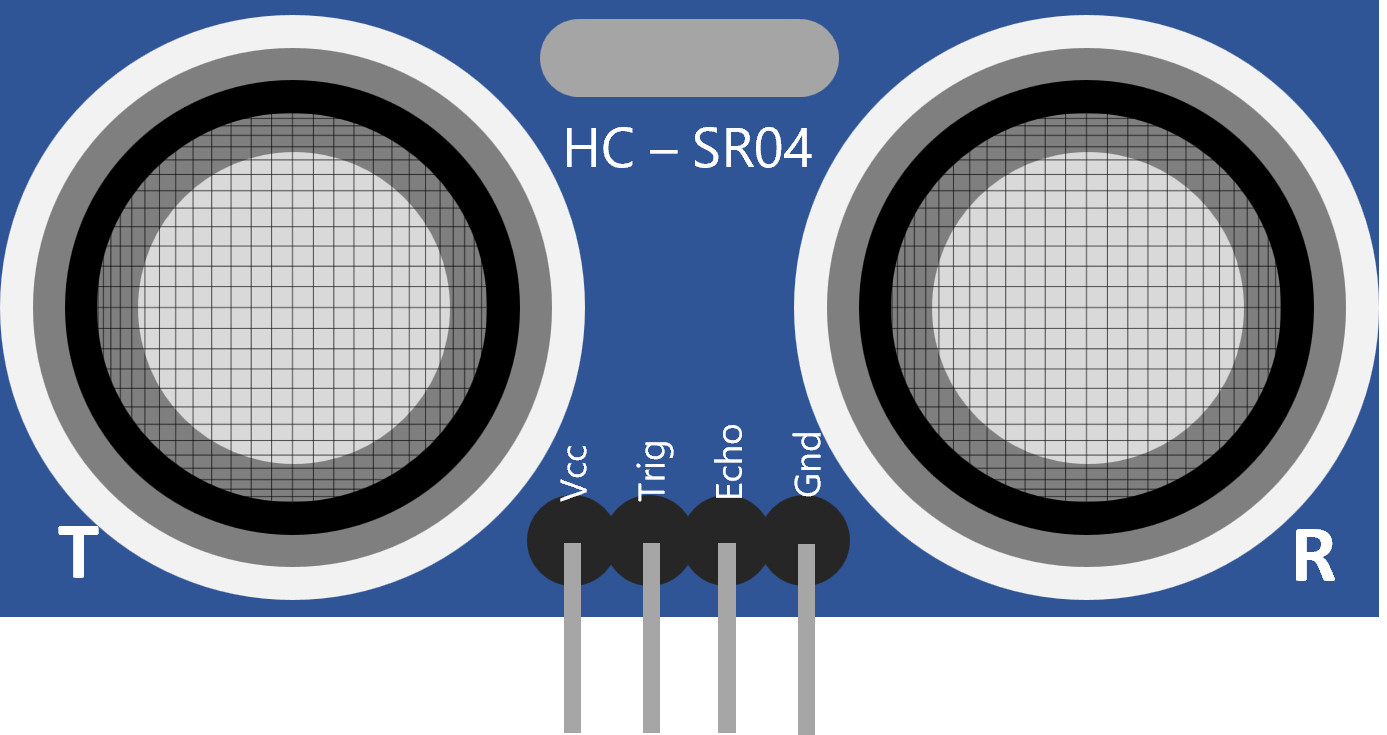
\includegraphics{images/HC-SR04_Sensor.png}
	}
	\caption[HC-SR04 Sensor Vorderseite]{HC-SR04 Sensor, Vorderseite, eigene Darstellung \protect\citeM{i}{IoTspace.dev}{}{}} \label{fig:withSource} % Wie gebe ich hier die Quelle an?
\end{figure}

Bei dem Sensor handelt es sich um einen auf Ultraschalltechnologie besierenden Distanzsensor. Er enthält einen Ultraschallsender sowie einen Ultrasschallempfänger und wird mit einer Spannung von 5V betrieben. Im Rahmen einer einzelnen Messung sendet der Ultaschallsender Ultraschallsignale aus. Der Ultraschallempfänger empfängt diese Signale und wandelt sie in ein elektrisches Signal um \protect\citeM{i}{HSHL.2023}{}{}.\\
Wenn das im rechten Sensor erzeugte Signal gemessen wird, kann die Zeit ermittelt werden, welche zwischen Absenden des Ultraschallsignals und dessen Wiederkehr liegt. Da die Geschwindigkeit vom Ultraschall durch Luft bekannt ist, kann die zurückgelegte Distanz und dadurch ebenso die Entfernung ermittelt werden. Hierzu wird die folgende Formel verwendet:\\\\
\begin{minipage}{\linewidth}
	\begin{equation}
		L {=} \frac{1}{2} \cdot T \cdot C
	\end{equation}
	\begin{tabular}{ll}
	L: & Distanz zum nächsten Objekt \\
	T: & Gemessene Zeit \\
	C: & Schallgeschwindigkeit
	\end{tabular}
\end{minipage}\\\\
Da der Sensor im Rahmen dieser Arbeit ausschließlich unter Normalbedingungen in Luft getestet wurde, kann die Schallgeschwindigkeit als nährungsweise Konstant angenommen werden. Mit diesem Wert lässt sich die Formel ergänzen:\\\\
\begin{minipage}{\linewidth}
	\begin{equation}
		L {=} \frac{343}{2} \cdot \frac{\text{m}}{\text{s}} \cdot T\\
	\end{equation}
	\begin{tabular}{ll}
	L: & Distanz zum nächsten Objekt \\
	T: & Gemessene Zeit
	\end{tabular}
\end{minipage}\\\\

\subsection{Ungenauigkeit und Messfehler}
\label{subsec:ungenauigkeit_und_messfehler}
Bei der Verwendung von Sensoren ist immer mit einer gewissen Ungenauigkeit der gemessenen Werte zu rechnen. Diese treten unweigerlich durch sich ständig ändernde äußere Faktoren auf, können jedoch ebenso durch eine falsche Verwendung des entsprechenden Sensors hervorgerufen werden.\\
Äußere Faktoren sind die Erdanziehungskraft, die Temperatur, das Material in dem der Sensor verwendet wird und viele weitere Faktoren. Beispielsweise hängt die Ausbreitungsgeschwindigkeit des Schalls von der Temperatur ab. Ist es extrem kalt, so breitet sich der Schall langsamer aus, als bei hohen Temperaturen \protect\citeM{i}{Raabe_Armin_Holstein_Peter.2021}{4}{5}.
Viel extremere Ausmaße haben oft Fehler bei der Verwendung des Sensors. Beispielsweise ist der HC-SR04 Sensor nur für das Messen von Distanzen zwischen 2 cm und 4 m ausgelegt. Wenn also Distanzen unter zwei Zentimetern oder über vier Metern gemessen werden, dann könnte ein Fehlerwert das Ergenis sein. Das liegt daran, dass der Sensor bei so geringen beziehungsweise hohen Distanzen das Signal nicht mehr erhält und nach einer geringen Wartezeit die Prüfung beendet, damit der Computer nicht dauerhaft auf eine Auflösung wartet. Für den HC-SR04 beläuft sich das Ergebnis einer Fehlmessung immer auf den Fehlerwert von acht Metern. In der Realität könnte ein solcher Fehlerwert natürlich weitreichende Auswirkungen haben. Ein einfaches Beispiel für die Auswirkungen einer Fehlmessung ohne Interpretation der Messwerte wäre das Parken eines Autos. Wenn sich sehr nah hinter dem Fahrzeug ein Fußgänger befindet und der Sensor aufgrund der geringen Distanz den Fehlerwert von acht Metern an den Fahrer weitergibt, so könnte dies im schlimmsten Falle tödlich für den Fußgänger enden.\\

\subsection{Interpretation von Messdaten}
Die Ungenauigkeit von Messergebnissen, ob durch äußere Einflüsse oder falsche Verwendung macht die reinen Messergenisse unnutzbar. Aus diesem Grund müssen die gemessenen Daten vor der Weitergabe an einen nicht Fachkundigen richtig interpretiert werden. Wie genau die 'richtige' Interpretation der Messdaten aussieht, hängt immer am entsprechenden Anwendungsgebiet und dem verwendeten Sensor.\\
Für den HC-SR04 können jegliche Werte zwischen zwei Zentimetern und vier Metern als realistische Werte angesehen und weitergegeben werden. Sobald ein Wert außerhalb dieses Bereichs gemessen wird, muss von einer potentiellen Messungenauigkeit ausgegangen werden. Der Wert darf nicht an den Nutzer weitergegeben werden. Besonders interessant sind beim HC-SR04 die Werte von knapp unter bis knapp über acht Metern. Diese bedeuten nämlich in der Regel immer, dass das gesendete Signal nicht wieder aufgenommen wurde. Wie bereits unter \ref{subsec:ungenauigkeit_und_messfehler} erwähnt, kann dieser Wert also ein extrem nahes, oder ein extrem weit entferntes Objekt indizieren. Der Umgang mit diesen Werten hängt von der Anwendung des Sensors ab. Befindet sich der Sensor an einem sich Bewegenden Objekt wie beispielsweise einem Fahrzeug und die Werte werden in einer hohen Frequenz mindestens einmalig jede Sekunde abgefragt, so kann man folgende Annahme treffen:\\
Waren die letzten Werte sehr nah an der unteren Grenze, so besteht große Gefahr einer Kollision. Man sollte von einem Minimalwert ausgehen. Waren die letzten Werte eher in der Nähe der oberen Grenze, so ist die Wahrscheinlichkeit sehr hoch, dass die Distanz sich weiter ausgebaut hat und das nächste Objekt sich nun außerhalb der Reichweite des Sensors befindet.\\
Wird der Sensor jedoch in einer Art Radar an einem sich drehenden Turm verwendet, so kann aus den letzten Werten kein Schluss auf den aktuellen Wert getroffen werden.

%\section{Anwendung von Abstandssensoren in der Automobilindustrie}
%\begin{itemize}
%    \item Ultraschallsensoren \\
%	Werden oftmals für Parkassistenten sowie Hinderniserkennung verwendet. Dieser Sensortyp eignet sich hierzu besonders aufgrund seines geringen Preises und der effektiven Messreichweite zwischen wenigen Zentimetern und einigen Metern.
%    \item \ac{LiDAR} \\
%	\ac{LiDAR}-Sensoren werden in modernen Fahrzeugen meist im \ac{ADAS} verwendet. Das \ac{ADAS} umfasst alle Systeme, welche den Fahrer durch Automatisierung unterstützen. Beispiele für solche Systeme sind Adaptives Fernlicht sowie Automatische Notbremsfunktion. Der \ac{LiDAR}-Sensor wird hierbei zum Erfassen einer Live-Umgebungskarte verwendet. Er eignet sich aus mehreren Gründen besonders gut für diese Aufgabe. Hierzu zählen seine Wetterbeständigkeit, die unabhängigkeit von Lichtverhältnissen bei der Messung sowie auch die hohe Präzision und Reichweite des Sensortyps.
%	\item DELETE \\
%	Quelle: https://www.bmw.com/de/innovation/sensoren-im-auto.html
%\end{itemize}

\section{Übertragung von Daten mittels eines Webservers}
Nachdem die Daten von einem Sensor erfasst wurden, können diese kurzzeitig ausgewertet und verwendet werden. Oftmals ist in modernen Anwendungen jedoch eine langfristige Auswertung der Daten, beispielweise aus Versicherungsgründen, notwendig. Im Rahmen des Hello World Projektes soll die Sicherung der Daten außerhalb des ermittelnden Systems ermöglicht werden. Die Vorgabe hierzu ist, dass der genutzte ESp einen Webserver starten soll, welcher einerseits die ermittelten Daten in sinnvollem Format zur Verfügung Stellt. Andererseits soll der Webserver auch eine Webseite Hosten, welche Echtzeitdaten für einen Benutzer transparent macht.

\subsection{OSI-Schichtenmodell}
Das \ac{OSI}-Schichtenmodell ein 1984 von der  \ac{ISO} entwickeltes Modell zur Aufteilung des Kommunikationsprozesses zwischen Computern in sieben Schichten. Diese Schichtunterteilung erleichtert die Kommunikation zwischen verschiedenen Computern. Die Kommunikation wird so Betriebssystemunabhängig und Implementationsunabhängig gewährleistet, solange beide Geräte sich an die im \ac{OSI}-Modell beschriebenen Vorgaben halten.

\subsubsection{Schichten des \ac{OSI}-Modells} 
\autoref{tab:tabelle_osi} zeigt die einzelnen Schichten des \ac{OSI}-Modells.
\begin{table}[h!]
	\centering
	\begin{tabular}{p{3cm}crl}
		\textbf{Schicht} & \textbf{\ac{OSI}-Schicht} &\textbf{\ac{OSI}-Layer (en)} \\\toprule
		VII &  Anwendungsschicht & Application Layer\\
		VI &  Darstellungsschicht & Presentation Layer\\
		V &  Kommunikationsschicht & Session Layer\\
		IV &  Transportschicht & Transport Layer\\
		III &  Vermittlungsschicht & Network Layer\\
		II &  Sicherungsschicht & Data Link Layer\\
		I &  Pysikalische Schicht & Physical Layer\\\bottomrule
	\end{tabular}
	\caption[\ac{OSI}-Schichten]{\label{tab:tabelle_osi}\ac{OSI}-Schichten}
\end{table}

\subsection{HTTP}
Da im Rahmen dieses Projektes mehrere Endpoints gehostet werden sollen, welche die Sensordaten bereitstellen, wird das \ac{HTTP}-Protokoll verwendet. Für die Kommunikation zwischen zwei PCs über das Internet wird fast ausschließlich dieses 1992 eingeführte Protokoll verwendet. \ac{HTTP}  standardisiert die Kommunikation zwischen den Anwendungsschichten (\ac{OSI}, \autoref{tab:tabelle_osi}) zweier Computer. Hierzu gibt es eine genaue Struktur vor, mit der Daten gesendet werden müssen. Beispielsweise muss der Typ der Anfrage als 'method' und die zu übertragenden Daten als 'body' angegeben werden. Darüber hinaus gibt es noch einige weitere Informationen, welche für die Übertragung per HTTP relevant sind.\\
\ac{HTTP} wird beispielsweise immer verwendet, wenn Webseiten in einem Internetbrowser geladen werden. Wenn hier eine neue Website geladen wird, dann erstellt dieser eine HTTP-Anfrage. Diese Anfrage nutzt den Anfragentyp 'GET', weil die Daten ja von diesem PC angefragt werden. Wenn der anfragende PC dann eine Antwort vom Server erhält, dann handelt es sich in der Regel um einen \ac{HTML}-Text. Dieser wird vom Browser erkannt und als Website dargestellt.\\
Ein großer Nachteil von \ac{HTTP} ist die fehlende Sicherheit der Technologie. Werden Daten nach den Standards dieses Protokolls übertragen, so sind sie nicht verschlüsselt und damit ebenso für jeden im Selben Netzwerk lesbar. Aus diesem Grund wurde das erstmals 1994 verwendete \ac{HTTPS} zum heutigen Standard für die Übertragug von Daten über das Internet. Dieses Protokoll funktioniert exakt wie dessen Vorbild \ac{HTTP}. Die einzige Anpassung ist, dass die Daten vor dem Absenden verschlüsselt und beim Empfänger anschließend wieder entschlüsselt werden. So kann jemand im Selben Netzwerk die Daten zwar erhalten und anschauen, jedoch nicht lesen. Hierzu würde er einen einzigartigen Schlüssel benötigen.\\
